\documentclass[twoside]{book}

% Packages required by doxygen
\usepackage{fixltx2e}
\usepackage{calc}
\usepackage{doxygen}
\usepackage[export]{adjustbox} % also loads graphicx
\usepackage{graphicx}
\usepackage[utf8]{inputenc}
\usepackage{makeidx}
\usepackage{multicol}
\usepackage{multirow}
\PassOptionsToPackage{warn}{textcomp}
\usepackage{textcomp}
\usepackage[nointegrals]{wasysym}
\usepackage[table]{xcolor}

% NLS support packages
\usepackage[brazil]{babel}
% Font selection
\usepackage[T1]{fontenc}
\usepackage[scaled=.90]{helvet}
\usepackage{courier}
\usepackage{amssymb}
\usepackage{sectsty}
\renewcommand{\familydefault}{\sfdefault}
\allsectionsfont{%
  \fontseries{bc}\selectfont%
  \color{darkgray}%
}
\renewcommand{\DoxyLabelFont}{%
  \fontseries{bc}\selectfont%
  \color{darkgray}%
}
\newcommand{\+}{\discretionary{\mbox{\scriptsize$\hookleftarrow$}}{}{}}

% Page & text layout
\usepackage{geometry}
\geometry{%
  a4paper,%
  top=2.5cm,%
  bottom=2.5cm,%
  left=2.5cm,%
  right=2.5cm%
}
\tolerance=750
\hfuzz=15pt
\hbadness=750
\setlength{\emergencystretch}{15pt}
\setlength{\parindent}{0cm}
\setlength{\parskip}{0.2cm}
\makeatletter
\renewcommand{\paragraph}{%
  \@startsection{paragraph}{4}{0ex}{-1.0ex}{1.0ex}{%
    \normalfont\normalsize\bfseries\SS@parafont%
  }%
}
\renewcommand{\subparagraph}{%
  \@startsection{subparagraph}{5}{0ex}{-1.0ex}{1.0ex}{%
    \normalfont\normalsize\bfseries\SS@subparafont%
  }%
}
\makeatother

% Headers & footers
\usepackage{fancyhdr}
\pagestyle{fancyplain}
\fancyhead[LE]{\fancyplain{}{\bfseries\thepage}}
\fancyhead[CE]{\fancyplain{}{}}
\fancyhead[RE]{\fancyplain{}{\bfseries\leftmark}}
\fancyhead[LO]{\fancyplain{}{\bfseries\rightmark}}
\fancyhead[CO]{\fancyplain{}{}}
\fancyhead[RO]{\fancyplain{}{\bfseries\thepage}}
\fancyfoot[LE]{\fancyplain{}{}}
\fancyfoot[CE]{\fancyplain{}{}}
\fancyfoot[RE]{\fancyplain{}{\bfseries\scriptsize Gerado em Domingo, 6 de Dezembro de 2015 03\+:00\+:24 para Ficha\+R\+P\+G por Doxygen }}
\fancyfoot[LO]{\fancyplain{}{\bfseries\scriptsize Gerado em Domingo, 6 de Dezembro de 2015 03\+:00\+:24 para Ficha\+R\+P\+G por Doxygen }}
\fancyfoot[CO]{\fancyplain{}{}}
\fancyfoot[RO]{\fancyplain{}{}}
\renewcommand{\footrulewidth}{0.4pt}
\renewcommand{\chaptermark}[1]{%
  \markboth{#1}{}%
}
\renewcommand{\sectionmark}[1]{%
  \markright{\thesection\ #1}%
}

% Indices & bibliography
\usepackage{natbib}
\usepackage[titles]{tocloft}
\setcounter{tocdepth}{3}
\setcounter{secnumdepth}{5}
\makeindex

% Hyperlinks (required, but should be loaded last)
\usepackage{ifpdf}
\ifpdf
  \usepackage[pdftex,pagebackref=true]{hyperref}
\else
  \usepackage[ps2pdf,pagebackref=true]{hyperref}
\fi
\hypersetup{%
  colorlinks=true,%
  linkcolor=blue,%
  citecolor=blue,%
  unicode%
}

% Custom commands
\newcommand{\clearemptydoublepage}{%
  \newpage{\pagestyle{empty}\cleardoublepage}%
}


%===== C O N T E N T S =====

\begin{document}

% Titlepage & ToC
\hypersetup{pageanchor=false,
             bookmarks=true,
             bookmarksnumbered=true,
             pdfencoding=unicode
            }
\pagenumbering{roman}
\begin{titlepage}
\vspace*{7cm}
\begin{center}%
{\Large Ficha\+R\+P\+G \\[1ex]\large 1.\+0 }\\
\vspace*{1cm}
{\large Gerado por Doxygen 1.8.10}\\
\vspace*{0.5cm}
{\small Domingo, 6 de Dezembro de 2015 03:00:24}\\
\end{center}
\end{titlepage}
\clearemptydoublepage
\tableofcontents
\clearemptydoublepage
\pagenumbering{arabic}
\hypersetup{pageanchor=true}

%--- Begin generated contents ---
\chapter{Namespaces}
\section{Lista de Namespaces}
Esta é a lista de todos os Namespaces com suas respectivas descrições\+:\begin{DoxyCompactList}
\item\contentsline{section}{\hyperlink{namespace_ui}{Ui} }{\pageref{namespace_ui}}{}
\end{DoxyCompactList}

\chapter{Índice Hierárquico}
\section{Hierarquia de Classes}
Esta lista de hierarquias está parcialmente ordenada (ordem alfabética)\+:\begin{DoxyCompactList}
\item Q\+Main\+Window\begin{DoxyCompactList}
\item \contentsline{section}{Main\+Window}{\pageref{class_main_window}}{}
\end{DoxyCompactList}
\end{DoxyCompactList}

\chapter{Índice dos Componentes}
\section{Lista de Componentes}
Aqui estão as classes, estruturas, uniões e interfaces e suas respectivas descrições\+:\begin{DoxyCompactList}
\item\contentsline{section}{\hyperlink{class_main_window}{Main\+Window} }{\pageref{class_main_window}}{}
\end{DoxyCompactList}

\chapter{Índice dos Arquivos}
\section{Lista de Arquivos}
Esta é a lista de todos os arquivos e suas respectivas descrições\+:\begin{DoxyCompactList}
\item\contentsline{section}{\hyperlink{main_8cpp}{main.\+cpp} }{\pageref{main_8cpp}}{}
\item\contentsline{section}{\hyperlink{mainwindow_8cpp}{mainwindow.\+cpp} }{\pageref{mainwindow_8cpp}}{}
\item\contentsline{section}{\hyperlink{mainwindow_8h}{mainwindow.\+h} }{\pageref{mainwindow_8h}}{}
\end{DoxyCompactList}

\chapter{Namespaces}
\hypertarget{namespace_ui}{}\section{Refência do Namespace Ui}
\label{namespace_ui}\index{Ui@{Ui}}


\subsection{Descrição Detalhada}
\hyperlink{mainwindow_8h}{Mainwindow.\+h} Autor Raphael Guedes Spinelli Versão 1.\+0 Data 2015 
\chapter{Classes}
\hypertarget{class_main_window}{}\section{Referência da Classe Main\+Window}
\label{class_main_window}\index{Main\+Window@{Main\+Window}}


{\ttfamily \#include $<$mainwindow.\+h$>$}

Diagrama de Hierarquia para Main\+Window\+:\begin{figure}[H]
\begin{center}
\leavevmode
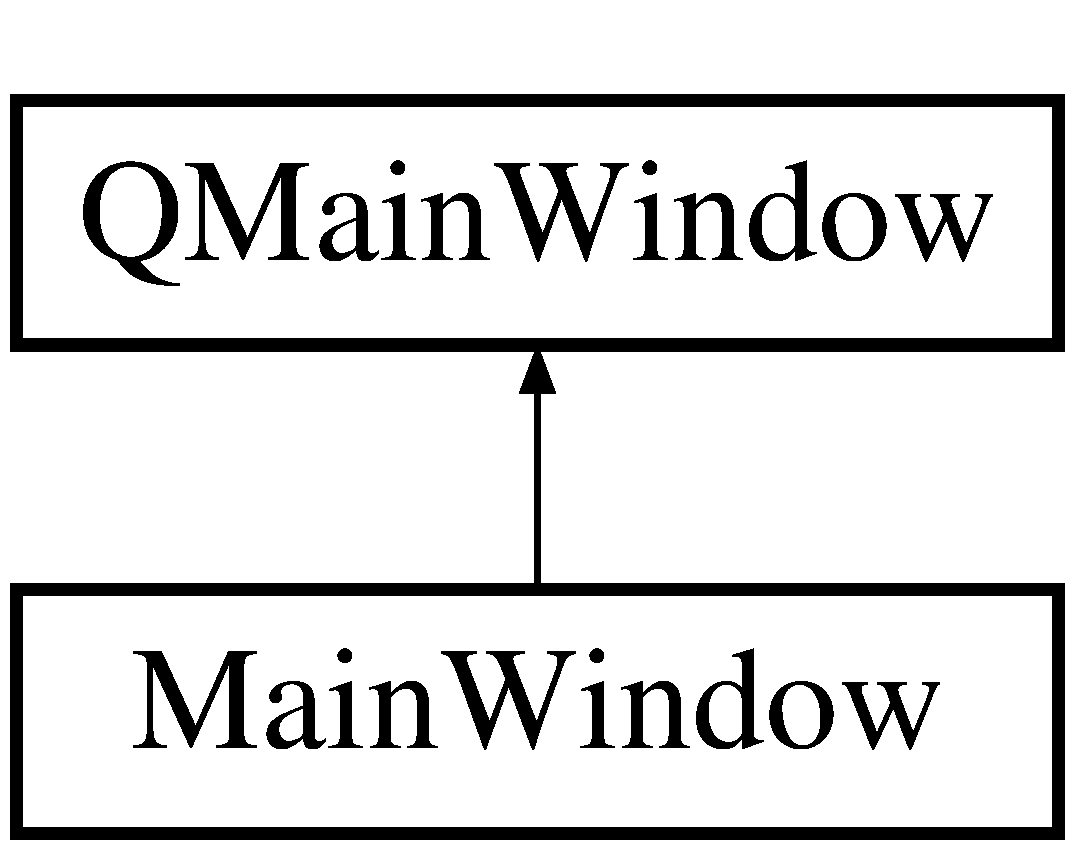
\includegraphics[height=2.000000cm]{class_main_window}
\end{center}
\end{figure}
\subsection*{Sinais}
\begin{DoxyCompactItemize}
\item 
void \hyperlink{class_main_window_a1f266c6dc033f3cd622a23526a707e3a}{mudar\+\_\+atributos\+Forca} (int)
\item 
void \hyperlink{class_main_window_a58c480645859287d0748f33db1ac6f01}{mudar\+\_\+atributos\+Destreza} (int)
\item 
void \hyperlink{class_main_window_a370f3a9d690ca64f1039fbfe0e53b245}{mudar\+\_\+atributos\+Inteligencia} (int)
\item 
void \hyperlink{class_main_window_ab0ecc3ebfbb38b4a3a775a614a84b785}{mudar\+\_\+atributos\+Constituicao} (int)
\item 
void \hyperlink{class_main_window_a5e98b6c94a1f5e469c242a0acd976155}{mudar\+\_\+atributos\+Carisma} (int)
\item 
void \hyperlink{class_main_window_ae85e30809106bb2c7517f0138931ff69}{pv} (int)
\item 
void \hyperlink{class_main_window_ad26f03bdbc050c7aafb9a980f860185c}{pm} (int)
\item 
void \hyperlink{class_main_window_a4d749e6affe917017b632bbc8e92255d}{pa} (int)
\item 
void \hyperlink{class_main_window_adcccf274033cd824252fba3eaba50049}{inic} (int)
\item 
void \hyperlink{class_main_window_ad0662ca7aff264d24250c5758f6a78aa}{vida\+\_\+atual} (int)
\item 
void \hyperlink{class_main_window_a1af874e03ad5046993b9a5d65d020eaa}{mana\+\_\+atual} (int)
\item 
void \hyperlink{class_main_window_a089e32820fe5916ab21d55f13db38658}{acao\+\_\+atual} (int)
\item 
void \hyperlink{class_main_window_a574a83ad071e949db94350382285a045}{dinheiro\+\_\+atual} (int)
\item 
void \hyperlink{class_main_window_a5493a7904845903c2cce21ec7e6b38a5}{pocao\+\_\+de\+\_\+vida\+\_\+atual} (int)
\item 
void \hyperlink{class_main_window_a9cd0839a3ca86169dd2ee0c34a495389}{pocao\+\_\+de\+\_\+mana\+\_\+atual} (int)
\end{DoxyCompactItemize}
\subsection*{Métodos Públicos}
\begin{DoxyCompactItemize}
\item 
\hyperlink{class_main_window_a8b244be8b7b7db1b08de2a2acb9409db}{Main\+Window} (Q\+Widget $\ast$parent=0)
\item 
\hyperlink{class_main_window_ae98d00a93bc118200eeef9f9bba1dba7}{$\sim$\+Main\+Window} ()
\item 
void \hyperlink{class_main_window_a4ce4094fd9e0e3fa1adf92431aba0890}{atulizar\+Dados} ()
\end{DoxyCompactItemize}


\subsection{Construtores \& Destrutores}
\hypertarget{class_main_window_a8b244be8b7b7db1b08de2a2acb9409db}{}\index{Main\+Window@{Main\+Window}!Main\+Window@{Main\+Window}}
\index{Main\+Window@{Main\+Window}!Main\+Window@{Main\+Window}}
\subsubsection[{Main\+Window(\+Q\+Widget $\ast$parent=0)}]{\setlength{\rightskip}{0pt plus 5cm}Main\+Window\+::\+Main\+Window (
\begin{DoxyParamCaption}
\item[{Q\+Widget $\ast$}]{parent = {\ttfamily 0}}
\end{DoxyParamCaption}
)\hspace{0.3cm}{\ttfamily [explicit]}}\label{class_main_window_a8b244be8b7b7db1b08de2a2acb9409db}
\hyperlink{mainwindow_8cpp}{Mainwindow.\+cpp} Autor Raphael Guedes Spinelli Versão 1.\+0 Data 2015 Variáveis que iniciam em Zero \hypertarget{class_main_window_ae98d00a93bc118200eeef9f9bba1dba7}{}\index{Main\+Window@{Main\+Window}!````~Main\+Window@{$\sim$\+Main\+Window}}
\index{````~Main\+Window@{$\sim$\+Main\+Window}!Main\+Window@{Main\+Window}}
\subsubsection[{$\sim$\+Main\+Window()}]{\setlength{\rightskip}{0pt plus 5cm}Main\+Window\+::$\sim$\+Main\+Window (
\begin{DoxyParamCaption}
{}
\end{DoxyParamCaption}
)}\label{class_main_window_ae98d00a93bc118200eeef9f9bba1dba7}


\subsection{Métodos}
\hypertarget{class_main_window_a089e32820fe5916ab21d55f13db38658}{}\index{Main\+Window@{Main\+Window}!acao\+\_\+atual@{acao\+\_\+atual}}
\index{acao\+\_\+atual@{acao\+\_\+atual}!Main\+Window@{Main\+Window}}
\subsubsection[{acao\+\_\+atual}]{\setlength{\rightskip}{0pt plus 5cm}void Main\+Window\+::acao\+\_\+atual (
\begin{DoxyParamCaption}
\item[{int}]{}
\end{DoxyParamCaption}
)\hspace{0.3cm}{\ttfamily [signal]}}\label{class_main_window_a089e32820fe5916ab21d55f13db38658}
Função que atualiza o valor da variavel pontos de ação atual chamada \char`\"{}vida\char`\"{}, recebe um valor inteiro \hypertarget{class_main_window_a4ce4094fd9e0e3fa1adf92431aba0890}{}\index{Main\+Window@{Main\+Window}!atulizar\+Dados@{atulizar\+Dados}}
\index{atulizar\+Dados@{atulizar\+Dados}!Main\+Window@{Main\+Window}}
\subsubsection[{atulizar\+Dados()}]{\setlength{\rightskip}{0pt plus 5cm}void Main\+Window\+::atulizar\+Dados (
\begin{DoxyParamCaption}
{}
\end{DoxyParamCaption}
)}\label{class_main_window_a4ce4094fd9e0e3fa1adf92431aba0890}
Função que atualiza as contas feitas pelo programa de acordo com as diferente variaveis \hypertarget{class_main_window_a574a83ad071e949db94350382285a045}{}\index{Main\+Window@{Main\+Window}!dinheiro\+\_\+atual@{dinheiro\+\_\+atual}}
\index{dinheiro\+\_\+atual@{dinheiro\+\_\+atual}!Main\+Window@{Main\+Window}}
\subsubsection[{dinheiro\+\_\+atual}]{\setlength{\rightskip}{0pt plus 5cm}void Main\+Window\+::dinheiro\+\_\+atual (
\begin{DoxyParamCaption}
\item[{int}]{}
\end{DoxyParamCaption}
)\hspace{0.3cm}{\ttfamily [signal]}}\label{class_main_window_a574a83ad071e949db94350382285a045}
Função que atualiza o valor da variavel dinheiro atual chamada \char`\"{}dinheiro\char`\"{}, recebe um valor inteiro \hypertarget{class_main_window_adcccf274033cd824252fba3eaba50049}{}\index{Main\+Window@{Main\+Window}!inic@{inic}}
\index{inic@{inic}!Main\+Window@{Main\+Window}}
\subsubsection[{inic}]{\setlength{\rightskip}{0pt plus 5cm}void Main\+Window\+::inic (
\begin{DoxyParamCaption}
\item[{int}]{}
\end{DoxyParamCaption}
)\hspace{0.3cm}{\ttfamily [signal]}}\label{class_main_window_adcccf274033cd824252fba3eaba50049}
Função que atualiza o valor da variavel iniciativa chamada \char`\"{}ini\char`\"{}, recebe um valor inteiro \hypertarget{class_main_window_a1af874e03ad5046993b9a5d65d020eaa}{}\index{Main\+Window@{Main\+Window}!mana\+\_\+atual@{mana\+\_\+atual}}
\index{mana\+\_\+atual@{mana\+\_\+atual}!Main\+Window@{Main\+Window}}
\subsubsection[{mana\+\_\+atual}]{\setlength{\rightskip}{0pt plus 5cm}void Main\+Window\+::mana\+\_\+atual (
\begin{DoxyParamCaption}
\item[{int}]{}
\end{DoxyParamCaption}
)\hspace{0.3cm}{\ttfamily [signal]}}\label{class_main_window_a1af874e03ad5046993b9a5d65d020eaa}
Função que atualiza o valor da variavel pontos de mana atual chamada \char`\"{}mana\char`\"{}, recebe um valor inteiro \hypertarget{class_main_window_a5e98b6c94a1f5e469c242a0acd976155}{}\index{Main\+Window@{Main\+Window}!mudar\+\_\+atributos\+Carisma@{mudar\+\_\+atributos\+Carisma}}
\index{mudar\+\_\+atributos\+Carisma@{mudar\+\_\+atributos\+Carisma}!Main\+Window@{Main\+Window}}
\subsubsection[{mudar\+\_\+atributos\+Carisma}]{\setlength{\rightskip}{0pt plus 5cm}void Main\+Window\+::mudar\+\_\+atributos\+Carisma (
\begin{DoxyParamCaption}
\item[{int}]{}
\end{DoxyParamCaption}
)\hspace{0.3cm}{\ttfamily [signal]}}\label{class_main_window_a5e98b6c94a1f5e469c242a0acd976155}
Função que atualiza o valor da variavel carisma chamada \char`\"{}car\char`\"{}, recebe um valor inteiro \hypertarget{class_main_window_ab0ecc3ebfbb38b4a3a775a614a84b785}{}\index{Main\+Window@{Main\+Window}!mudar\+\_\+atributos\+Constituicao@{mudar\+\_\+atributos\+Constituicao}}
\index{mudar\+\_\+atributos\+Constituicao@{mudar\+\_\+atributos\+Constituicao}!Main\+Window@{Main\+Window}}
\subsubsection[{mudar\+\_\+atributos\+Constituicao}]{\setlength{\rightskip}{0pt plus 5cm}void Main\+Window\+::mudar\+\_\+atributos\+Constituicao (
\begin{DoxyParamCaption}
\item[{int}]{}
\end{DoxyParamCaption}
)\hspace{0.3cm}{\ttfamily [signal]}}\label{class_main_window_ab0ecc3ebfbb38b4a3a775a614a84b785}
Função que atualiza o valor da variavel constituição chamada \char`\"{}cons\char`\"{}, recebe um valor inteiro \hypertarget{class_main_window_a58c480645859287d0748f33db1ac6f01}{}\index{Main\+Window@{Main\+Window}!mudar\+\_\+atributos\+Destreza@{mudar\+\_\+atributos\+Destreza}}
\index{mudar\+\_\+atributos\+Destreza@{mudar\+\_\+atributos\+Destreza}!Main\+Window@{Main\+Window}}
\subsubsection[{mudar\+\_\+atributos\+Destreza}]{\setlength{\rightskip}{0pt plus 5cm}void Main\+Window\+::mudar\+\_\+atributos\+Destreza (
\begin{DoxyParamCaption}
\item[{int}]{}
\end{DoxyParamCaption}
)\hspace{0.3cm}{\ttfamily [signal]}}\label{class_main_window_a58c480645859287d0748f33db1ac6f01}
Função que atualiza o valor da variavel destreza chamada \char`\"{}des\char`\"{}, recebe um valor inteiro \hypertarget{class_main_window_a1f266c6dc033f3cd622a23526a707e3a}{}\index{Main\+Window@{Main\+Window}!mudar\+\_\+atributos\+Forca@{mudar\+\_\+atributos\+Forca}}
\index{mudar\+\_\+atributos\+Forca@{mudar\+\_\+atributos\+Forca}!Main\+Window@{Main\+Window}}
\subsubsection[{mudar\+\_\+atributos\+Forca}]{\setlength{\rightskip}{0pt plus 5cm}void Main\+Window\+::mudar\+\_\+atributos\+Forca (
\begin{DoxyParamCaption}
\item[{int}]{}
\end{DoxyParamCaption}
)\hspace{0.3cm}{\ttfamily [signal]}}\label{class_main_window_a1f266c6dc033f3cd622a23526a707e3a}
Função que atualiza o valor da variavel força chamada \char`\"{}forc\char`\"{}, recebe um valor inteiro \hypertarget{class_main_window_a370f3a9d690ca64f1039fbfe0e53b245}{}\index{Main\+Window@{Main\+Window}!mudar\+\_\+atributos\+Inteligencia@{mudar\+\_\+atributos\+Inteligencia}}
\index{mudar\+\_\+atributos\+Inteligencia@{mudar\+\_\+atributos\+Inteligencia}!Main\+Window@{Main\+Window}}
\subsubsection[{mudar\+\_\+atributos\+Inteligencia}]{\setlength{\rightskip}{0pt plus 5cm}void Main\+Window\+::mudar\+\_\+atributos\+Inteligencia (
\begin{DoxyParamCaption}
\item[{int}]{}
\end{DoxyParamCaption}
)\hspace{0.3cm}{\ttfamily [signal]}}\label{class_main_window_a370f3a9d690ca64f1039fbfe0e53b245}
Função que atualiza o valor da variavel inteligência chamada \char`\"{}inte\char`\"{}, recebe um valor inteiro \hypertarget{class_main_window_a4d749e6affe917017b632bbc8e92255d}{}\index{Main\+Window@{Main\+Window}!pa@{pa}}
\index{pa@{pa}!Main\+Window@{Main\+Window}}
\subsubsection[{pa}]{\setlength{\rightskip}{0pt plus 5cm}void Main\+Window\+::pa (
\begin{DoxyParamCaption}
\item[{int}]{}
\end{DoxyParamCaption}
)\hspace{0.3cm}{\ttfamily [signal]}}\label{class_main_window_a4d749e6affe917017b632bbc8e92255d}
Função que atualiza o valor da variavel pontos de ação máximos chamada \char`\"{}pacao\char`\"{}, recebe um valor inteiro \hypertarget{class_main_window_ad26f03bdbc050c7aafb9a980f860185c}{}\index{Main\+Window@{Main\+Window}!pm@{pm}}
\index{pm@{pm}!Main\+Window@{Main\+Window}}
\subsubsection[{pm}]{\setlength{\rightskip}{0pt plus 5cm}void Main\+Window\+::pm (
\begin{DoxyParamCaption}
\item[{int}]{}
\end{DoxyParamCaption}
)\hspace{0.3cm}{\ttfamily [signal]}}\label{class_main_window_ad26f03bdbc050c7aafb9a980f860185c}
Função que atualiza o valor da variavel pontos de mana máximos chamada \char`\"{}pmana\char`\"{}, recebe um valor inteiro \hypertarget{class_main_window_a9cd0839a3ca86169dd2ee0c34a495389}{}\index{Main\+Window@{Main\+Window}!pocao\+\_\+de\+\_\+mana\+\_\+atual@{pocao\+\_\+de\+\_\+mana\+\_\+atual}}
\index{pocao\+\_\+de\+\_\+mana\+\_\+atual@{pocao\+\_\+de\+\_\+mana\+\_\+atual}!Main\+Window@{Main\+Window}}
\subsubsection[{pocao\+\_\+de\+\_\+mana\+\_\+atual}]{\setlength{\rightskip}{0pt plus 5cm}void Main\+Window\+::pocao\+\_\+de\+\_\+mana\+\_\+atual (
\begin{DoxyParamCaption}
\item[{int}]{}
\end{DoxyParamCaption}
)\hspace{0.3cm}{\ttfamily [signal]}}\label{class_main_window_a9cd0839a3ca86169dd2ee0c34a495389}
Função que atualiza o valor da variavel quantidade de poções de mana atual chamada \char`\"{}pocaom\char`\"{}, recebe um valor inteiro \hypertarget{class_main_window_a5493a7904845903c2cce21ec7e6b38a5}{}\index{Main\+Window@{Main\+Window}!pocao\+\_\+de\+\_\+vida\+\_\+atual@{pocao\+\_\+de\+\_\+vida\+\_\+atual}}
\index{pocao\+\_\+de\+\_\+vida\+\_\+atual@{pocao\+\_\+de\+\_\+vida\+\_\+atual}!Main\+Window@{Main\+Window}}
\subsubsection[{pocao\+\_\+de\+\_\+vida\+\_\+atual}]{\setlength{\rightskip}{0pt plus 5cm}void Main\+Window\+::pocao\+\_\+de\+\_\+vida\+\_\+atual (
\begin{DoxyParamCaption}
\item[{int}]{}
\end{DoxyParamCaption}
)\hspace{0.3cm}{\ttfamily [signal]}}\label{class_main_window_a5493a7904845903c2cce21ec7e6b38a5}
Função que atualiza o valor da variavel quantidade de poções de vida atual chamada \char`\"{}pocaov\char`\"{}, recebe um valor inteiro \hypertarget{class_main_window_ae85e30809106bb2c7517f0138931ff69}{}\index{Main\+Window@{Main\+Window}!pv@{pv}}
\index{pv@{pv}!Main\+Window@{Main\+Window}}
\subsubsection[{pv}]{\setlength{\rightskip}{0pt plus 5cm}void Main\+Window\+::pv (
\begin{DoxyParamCaption}
\item[{int}]{}
\end{DoxyParamCaption}
)\hspace{0.3cm}{\ttfamily [signal]}}\label{class_main_window_ae85e30809106bb2c7517f0138931ff69}
Função que atualiza o valor da variavel pontos de vida máximos chamada \char`\"{}pvida\char`\"{}, recebe um valor inteiro \hypertarget{class_main_window_ad0662ca7aff264d24250c5758f6a78aa}{}\index{Main\+Window@{Main\+Window}!vida\+\_\+atual@{vida\+\_\+atual}}
\index{vida\+\_\+atual@{vida\+\_\+atual}!Main\+Window@{Main\+Window}}
\subsubsection[{vida\+\_\+atual}]{\setlength{\rightskip}{0pt plus 5cm}void Main\+Window\+::vida\+\_\+atual (
\begin{DoxyParamCaption}
\item[{int}]{}
\end{DoxyParamCaption}
)\hspace{0.3cm}{\ttfamily [signal]}}\label{class_main_window_ad0662ca7aff264d24250c5758f6a78aa}
Função que atualiza o valor da variavel pontos de vida atual chamada \char`\"{}vida\char`\"{}, recebe um valor inteiro 

A documentação para esta classe foi gerada a partir dos seguintes arquivos\+:\begin{DoxyCompactItemize}
\item 
\hyperlink{mainwindow_8h}{mainwindow.\+h}\item 
\hyperlink{mainwindow_8cpp}{mainwindow.\+cpp}\end{DoxyCompactItemize}

\chapter{Arquivos}
\hypertarget{main_8cpp}{}\section{Referência do Arquivo main.\+cpp}
\label{main_8cpp}\index{main.\+cpp@{main.\+cpp}}
{\ttfamily \#include \char`\"{}mainwindow.\+h\char`\"{}}\\*
{\ttfamily \#include $<$Q\+Application$>$}\\*
\subsection*{Funções}
\begin{DoxyCompactItemize}
\item 
int \hyperlink{main_8cpp_a0ddf1224851353fc92bfbff6f499fa97}{main} (int argc, char $\ast$argv\mbox{[}$\,$\mbox{]})
\end{DoxyCompactItemize}


\subsection{Funções}
\hypertarget{main_8cpp_a0ddf1224851353fc92bfbff6f499fa97}{}\index{main.\+cpp@{main.\+cpp}!main@{main}}
\index{main@{main}!main.\+cpp@{main.\+cpp}}
\subsubsection[{main(int argc, char $\ast$argv[])}]{\setlength{\rightskip}{0pt plus 5cm}int main (
\begin{DoxyParamCaption}
\item[{int}]{argc, }
\item[{char $\ast$}]{argv\mbox{[}$\,$\mbox{]}}
\end{DoxyParamCaption}
)}\label{main_8cpp_a0ddf1224851353fc92bfbff6f499fa97}

\hypertarget{mainwindow_8cpp}{}\section{Referência do Arquivo mainwindow.\+cpp}
\label{mainwindow_8cpp}\index{mainwindow.\+cpp@{mainwindow.\+cpp}}
{\ttfamily \#include \char`\"{}mainwindow.\+h\char`\"{}}\\*
{\ttfamily \#include \char`\"{}ui\+\_\+mainwindow.\+h\char`\"{}}\\*

\hypertarget{mainwindow_8h}{}\section{Referência do Arquivo mainwindow.\+h}
\label{mainwindow_8h}\index{mainwindow.\+h@{mainwindow.\+h}}
{\ttfamily \#include $<$Q\+Main\+Window$>$}\\*
\subsection*{Componentes}
\begin{DoxyCompactItemize}
\item 
class \hyperlink{class_main_window}{Main\+Window}
\end{DoxyCompactItemize}
\subsection*{Namespaces}
\begin{DoxyCompactItemize}
\item 
 \hyperlink{namespace_ui}{Ui}
\end{DoxyCompactItemize}

%--- End generated contents ---

% Index
\backmatter
\newpage
\phantomsection
\clearemptydoublepage
\addcontentsline{toc}{chapter}{Índice}
\printindex

\end{document}
